
\chapter{\IfLanguageName{dutch}{Praktische uitvoering van ANPR}{Implementation of ANPR at UGent}}
\label{ch:praktischeUitvoering}
In dit hoofdstuk zal er onderzocht worden of nummerplaatdetectie degelijke resultaten kan leveren op de Campus Sterre en Campus Coupure van UGent. Hiervoor zullen handmatig foto's genomen worden van wagens die de parking willen verlaten met de Pi-NoIR cam. Hierna wordt er gecontroleerd of OpenANPR wel degelijk correcte resultaten levert op de genomen foto's.


\section{Hardware en software}
In dit onderdeel wordt de opstelling en configuratie van de camera's uitgelegd adhv. de informatie verzameld in Hoofdstuk \ref{ch:maatregelenanpr}.

\subsection{Camera}
Als camera zal gebruik gemaakt worden van de PiNoIR-Cam. Deze camera is een standaard extensie voor de Raspberry-PI die geen infrarood filtering heeft staan. Standaard wordt infrarood uit afbeeldingen gefilterd omdat deze een ongewenst bijproduct zijn op foto's. De PiNoIR camera filtert geen infrarood uit de afbeeldingen en maken het dus mogelijk om te gebruiken voor infrarood detectie.

\paragraph{Cameraplaatsing}
Voor de plaatsing van de camera's wordt er gewenst zo veel mogelijk kosten te besparen en wordt er liever niet geopteerd voor een aparte paal voor de ANPR-camera. Daarom zal als fotopunt de metalen constructie van de hefboom gekozen worden. De camera zal hier op de top worden aangehangen zodat deze zo min mogelijk interferentie heeft van de koplampen van de auto's.

\begin{figure}[h!]
	\centering
	\includegraphics[width=\linewidth]{img/uitgang-coupure.jpg}
	\caption{Uitgang met tokens aan UGent campus Coupure}
\end{figure}

\paragraph{Cameraconfiguratie}
De voorgaande camerainstellingen zullen zo correct mogelijk op de PiNoIR camera worden ingesteld.
TODO: configuratie bepalen
%TODO alpr commando's


\subsection{Opstelling}
Om de foto's te verkrijgen zal gebruik gemaakt worden van de Raspberry Pi met de PiNoIR camera, deze zal in een behuizing op de juiste hoogte van de paal tijdelijk vastgezet worden tesamen met een powerbank. De Raspberry Pi verbindt vervolgens met een GSM die als hotspot ingesteld staat, waarop vervolgens met een SSH verbinding een commando kan worden uitgevoerd om foto's te nemen.

Figuur \ref{Opstelling} toont de gemaakte opstelling. Deze bevat De Raspberry Pi, de Pi-Cam en een powerbank met een capaciteit van 700mAh.
\begin{figure}[h]
	\centering
	\includegraphics[width=0.5\linewidth]{img/camera.jpg}
	\caption{Opstelling Raspberry Pi met PiCam.}
	\label{Opstelling}
\end{figure}

\section{Verzamelen van de gegevens}

Om een correcte dataset te bekomen zal er op de parking van UGent zelf data verzameld worden aan de uitgangen.
Deze uitgangen zijn:
\begin{itemize}
	\item Campus Coupure - Uitgang Coupure Links
	\item Campus Coupure - Uitgang Kruisboogstraat
	\item Campus Landbouw - Uitgang De Pintelaan
	\item Campus Landbouw - Uitgang Galglaan
\end{itemize}

Per auto die de parking wilt verlaten worden er 6 foto's gemaakt in een periode van 3 seconden. Deze worden niet automatisch getriggerd, maar handmatig aan de hand van een SSH verbinding. Foto's die te laat of te vroeg werden genomen worden weggelaten. Enkele voorbeelden hiervan zijn te zien in Figuur \ref{fig:badpics}. Vervolgens wordt er per auto maar 1 foto bijgehouden per afstand. Indien er maar 1 afstand aanwezig is op de foto's, wordt deze reeks niet gezien als representatief en zullen de auto's niet verwerkt worden.

\begin{figure}[h!]
	\centering
	\begin{subfigure}[b]{0.45\linewidth}
		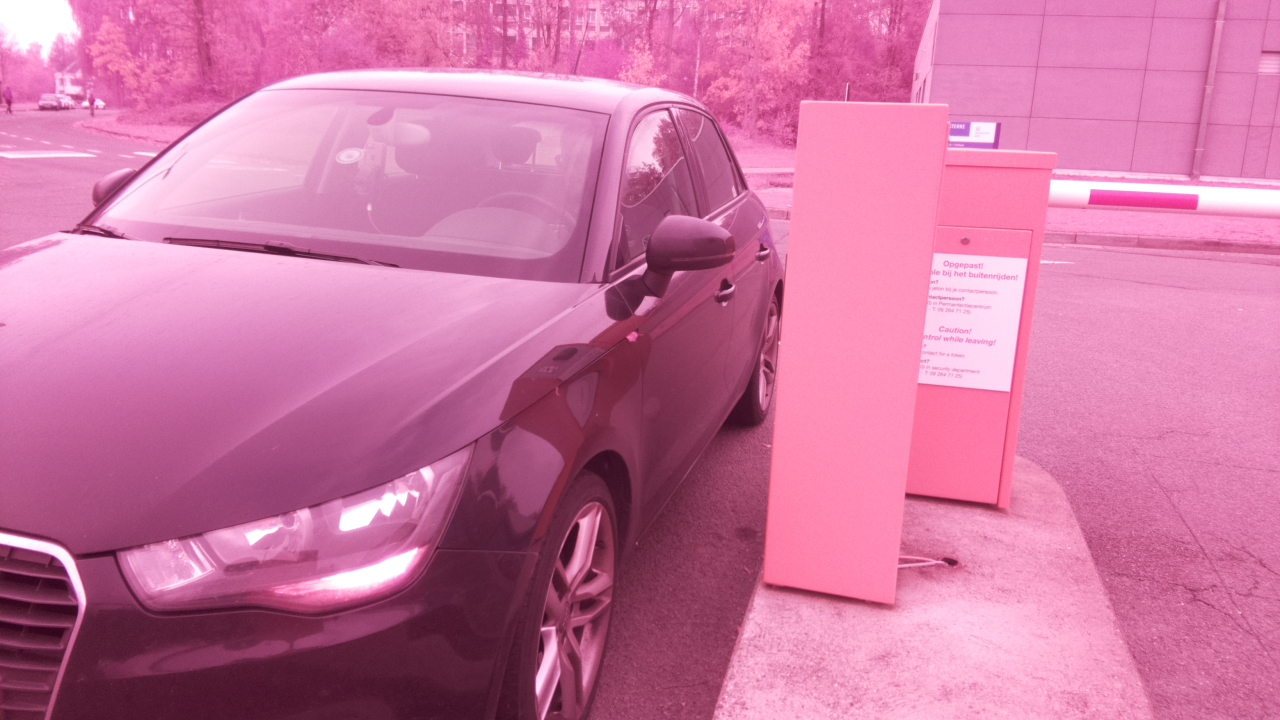
\includegraphics[width=\linewidth]{img/slecht/close.jpg}
		\caption{Auto op een onredelijk dichte afstand.}
	\end{subfigure}
	\begin{subfigure}[b]{0.45\linewidth}
		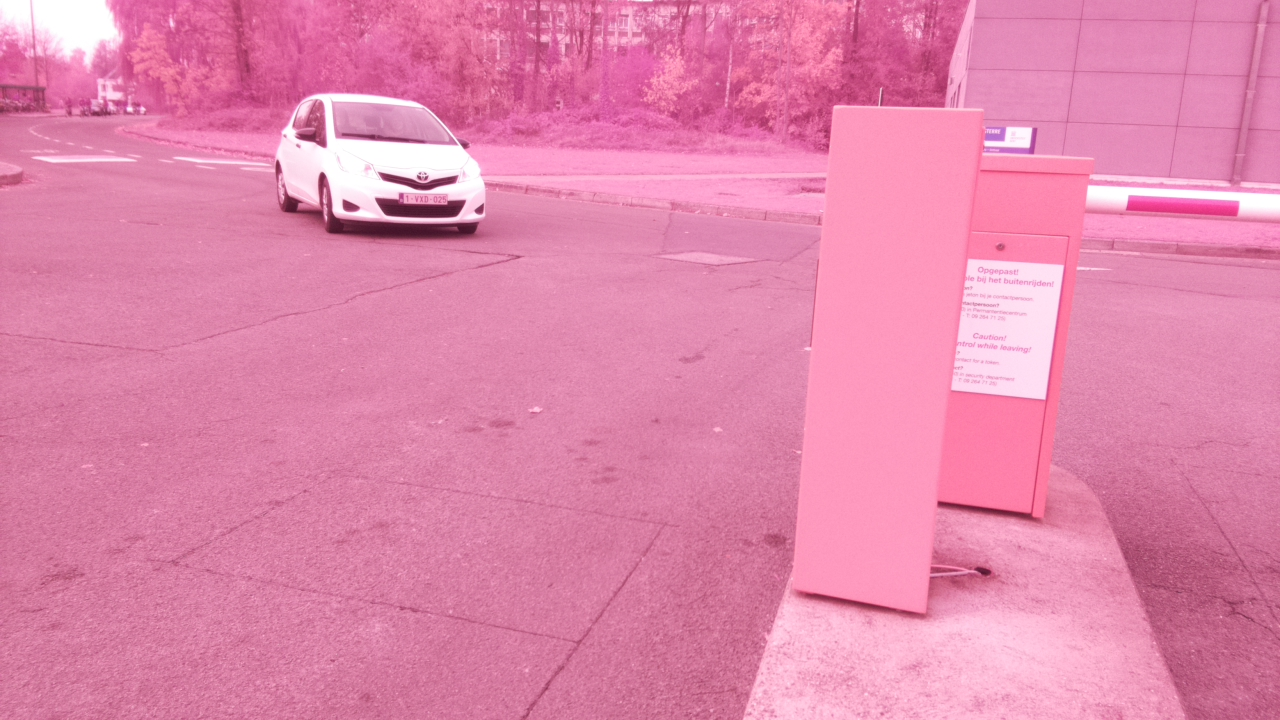
\includegraphics[width=\linewidth]{img/slecht/far.jpg}
		\caption{Auto op een onredelijk verre afstand.}
	\end{subfigure}
	\begin{subfigure}[b]{0.45\linewidth}
	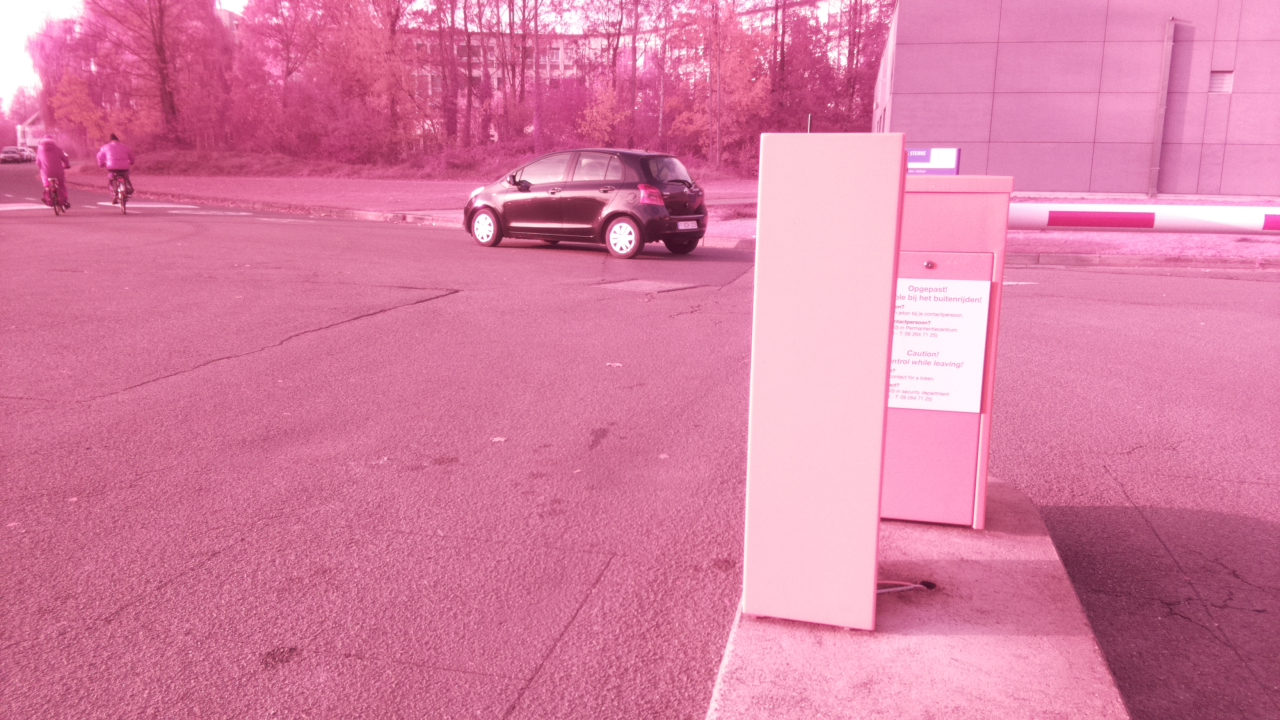
\includegraphics[width=\linewidth]{img/slecht/anderekant.jpg}
	\caption{Auto die de parking niet verlaat.}
	\end{subfigure}
	\caption{Types van foto's die niet opgenomen worden in het onderzoek.}
	\label{fig:badpics}
\end{figure}

In sommige gevallen zijn de foto's allemaal van een veel te verre afstand genomen, dit is niet representatief aangezien een motion detection systeem foto's over een korte afstand kan nemen. In het geval van Figuur \ref{fig:onlyfar} zijn alle afbeeldingen op een verre afstand genomen. Een motion detection systeem zou in dit geval ook foto's genomen kunnen hebben op een dichtere afstand, hierdoor is deze reeks foto's niet representatief en zal ook helemaal niet opgenomen worden in het onderzoek.
\begin{figure}[h!]
	\centering
	\begin{subfigure}[b]{0.45\linewidth}
		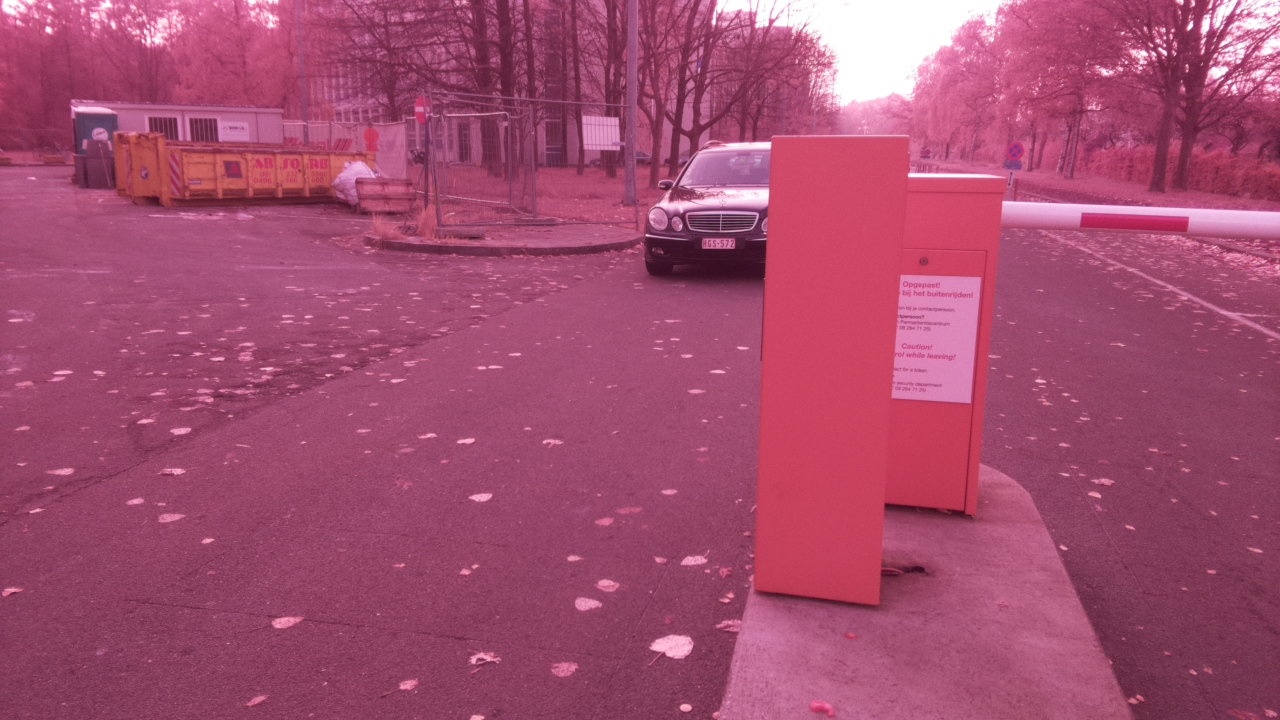
\includegraphics[width=\linewidth]{img/slecht/onlyfar1.jpg}
	\end{subfigure}
	\begin{subfigure}[b]{0.45\linewidth}
		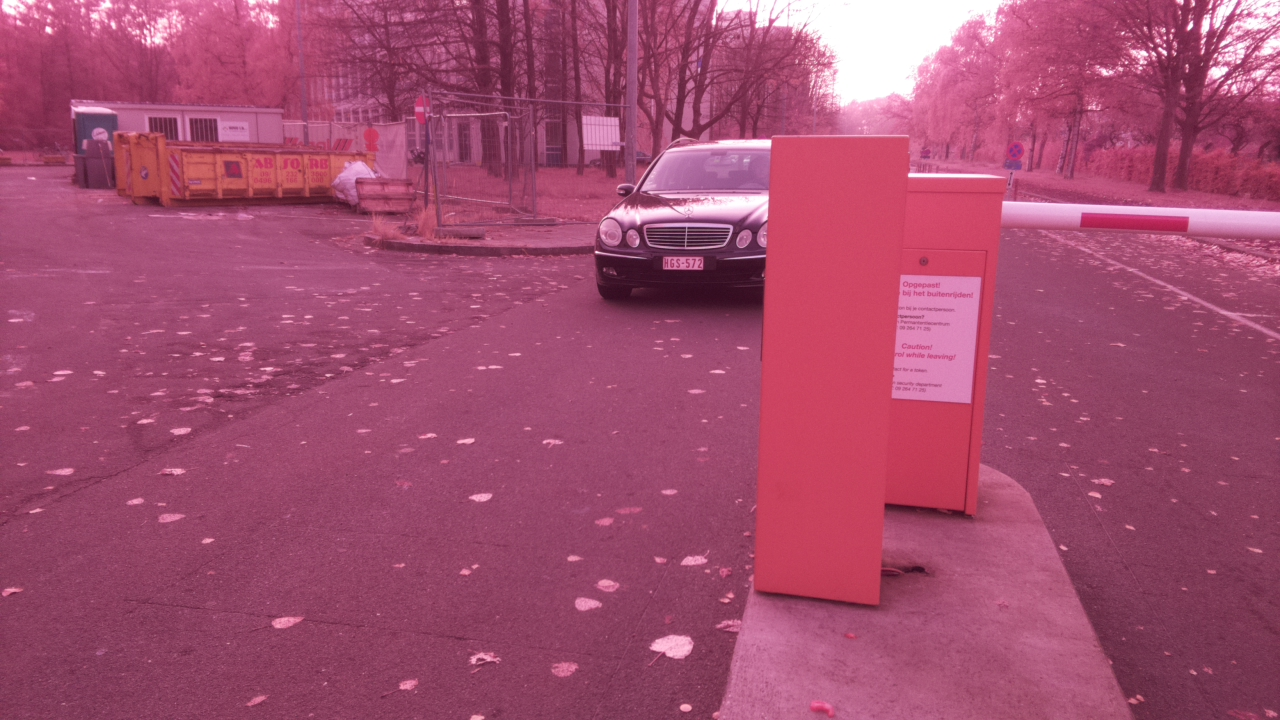
\includegraphics[width=\linewidth]{img/slecht/onlyfar2.jpg}
	\end{subfigure}
	\begin{subfigure}[b]{0.45\linewidth}
		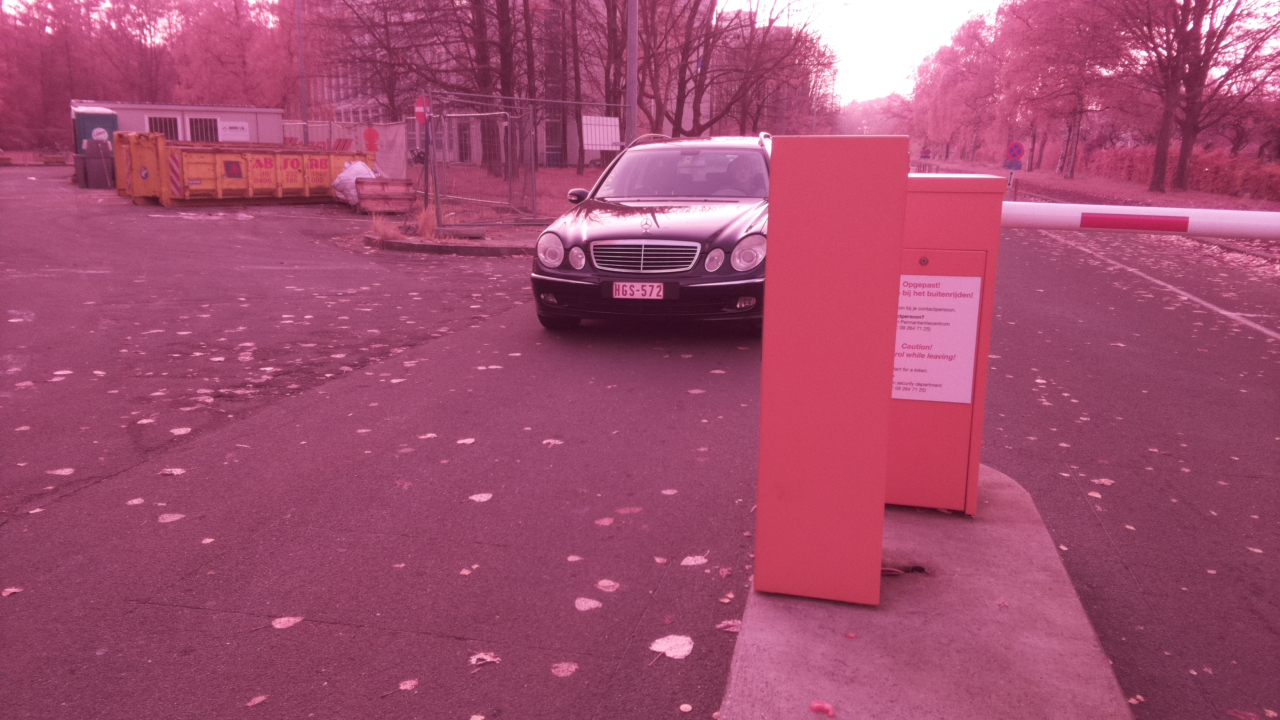
\includegraphics[width=\linewidth]{img/slecht/onlyfar3.jpg}
	\end{subfigure}
	\caption{Foto's die allemaal op een verre afstand genomen zijn en hierdoor dus niet representatief zijn.}
	\label{fig:onlyfar}
\end{figure}

Op volgende momenten en locaties zijn de foto's verzameld:
%TODO fix aantallen
\begin{table}[h]
\centering
\begin{tabular}{l|l|l|l|l}
	Datum 		& Begin & Eind	& Locatie	& Aantal foto's \\ \hline
	06/11/2019	& 11u45 & 12u46	& Campus Coupure - Uitgang Kruisboogstraat	& 53	\\
	08/11/2019	& 12u15 & 12u29	& Campus Sterre - Uitgang Galglaan	& 22	\\
	08/11/2019	& 12u52 & 13u41	& Campus Sterre - Uitgang De Pintelaan	& 38	\\
	13/11/2019	& 11u36 & 12u08	& Campus Sterre - Uitgang De Pintelaan	& 50	\\
	13/11/2019	& 12u29 & 12u42	& Campus Sterre - Uitgang Galglaan	& 10	\\
	13/11/2019	& 13u48 & 14u35	& Campus Coupure - Uitgang Coupure Links	& 5	\\
	14/11/2019	& 18u05 & 18u55	& Campus Coupure - Uitgang Coupure Links	& 3	\\
	21/11/2019	& 14u08 & 15u11	& Campus Sterre - Uitgang De Pintelaan	& 35	\\
	21/11/2019	& 15u58 & 16u22	& Campus Sterre - Uitgang Galglaan	& 36	\\
	27/11/2019	& 13u42 & 15u03	& Campus Sterre - Uitgang De Pintelaan	& 76	\\
\end{tabular}
\end{table}

Zo bekomen we volgende aantallen van foto's per uitgang:
\begin{table}[h]
	\centering
	\begin{tabular}{l|l}
		Uitgang	& Aantal foto's \\ \hline
		Campus Coupure - Uitgang Kruisboogstraat	& 53\\
		Campus Coupure - Uigang Coupure Links	& 5\\
		Campus Sterre - Uitgang Galglaan	& 32\\
		Campus Sterre - Uitgang De Pintelaan, camerahoek rechts	& 38\\
		Campus Sterre - Uitgang De Pintelaan, camerahoek links	& 50\\
	\end{tabular}
\end{table}

Per nummerplaat wordt volgende data genoteerd:
\begin{itemize}
	\item \textbf{identifier:} Unieke identifier per auto.
	\item \textbf{file:} De bestandsnaam van de foto.
	\item \textbf{license\_plate:} De 'correcte' nummerplaat, handmatig uit de foto gehaald.
	\item \textbf{result:} De nummerplaat gedetecteerd door OpenALPR.
	\item \textbf{distance:} De afstand van de camera, bestaat uit 3 velden, "close", "medium"\ en "far". Close betekent een afstand onder de 3 meter, medium tussen 3 en 5 meter en far betekent verder dan 5 meter.
	\item \textbf{lighting:} De belichting van de nummerplaten, bestaat uit 2 velden, "bright"\ en "very\_bright". Bright betekent dat de nummerplaat duidelijk leesbaar is voor mensen onder normaal daglicht. very\_bright betekent dat deze niet onmiddelijk leesbaar is.
	\item \textbf{location:} De uitgang waar de foto is genomen, bestaat uit "coupure-kruisboogstraat", "coupure-coupurelinks", "sterre-galglaan"\ en "sterre-depintelaan".
\end{itemize}

\section{Verwerking van gegevens}

Na de foto's gemaakt zijn worden deze geclassificeerd volgens nummerplaat, belichting, locatie en afstand van de camera. Vervo wordt er een automatische triggering van de camera's gebruikt.lgens wordt er nummerplaatdetectie uitgevoerd met behulp van OpenALPR en worden worden deze bij de bij de foto opgeslaan.

Per auto worden 2-3 foto's bijgehouden, deze worden geselecteerd op basis van de afstand. De auto dient op minstens 2 verschillende afstanden gedetecteert te zijn, dit om te voorkomen dat foto's van onrepresentabele afstanden genomen zijn. Het nemen van de foto's gebeurt via een handmatige trigger en heeft dus de mogelijkheid dat de foto's niet op een representabele afstand zijn. In een volledige implementatie zou de Raspberry Pi detecteren dat er beweging in de afbeelding is en automatisch triggeren.

De detectie van een nummerplaat is succesvol indien één van de genomen foto's correct is.
twee afstanden per auto.

\subsection{Calibratie van de afbeeldingen}
Origineel waren alle resultaten van de nummerplaatdetectie aan de zeer lage kant, aangezien de afbeeldingen nog niet gecalibreerd waren. Dit is beschreven in 
\begin{figure}[h!]
	\centering
	\begin{subfigure}[b]{0.4\linewidth}
		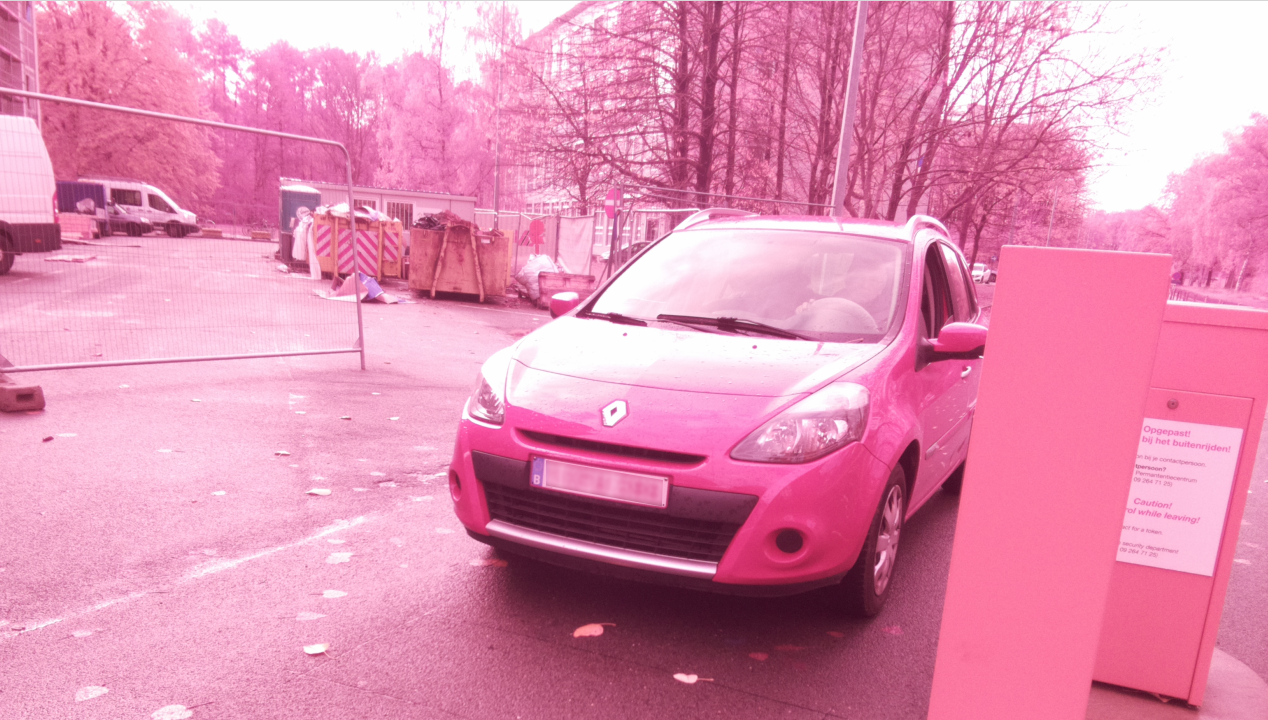
\includegraphics[width=\linewidth]{img/calibration/pre-calibrate.png}
		\caption{Niet-gekalibreerde afbeelding}
	\end{subfigure}
	\begin{subfigure}[b]{0.4\linewidth}
		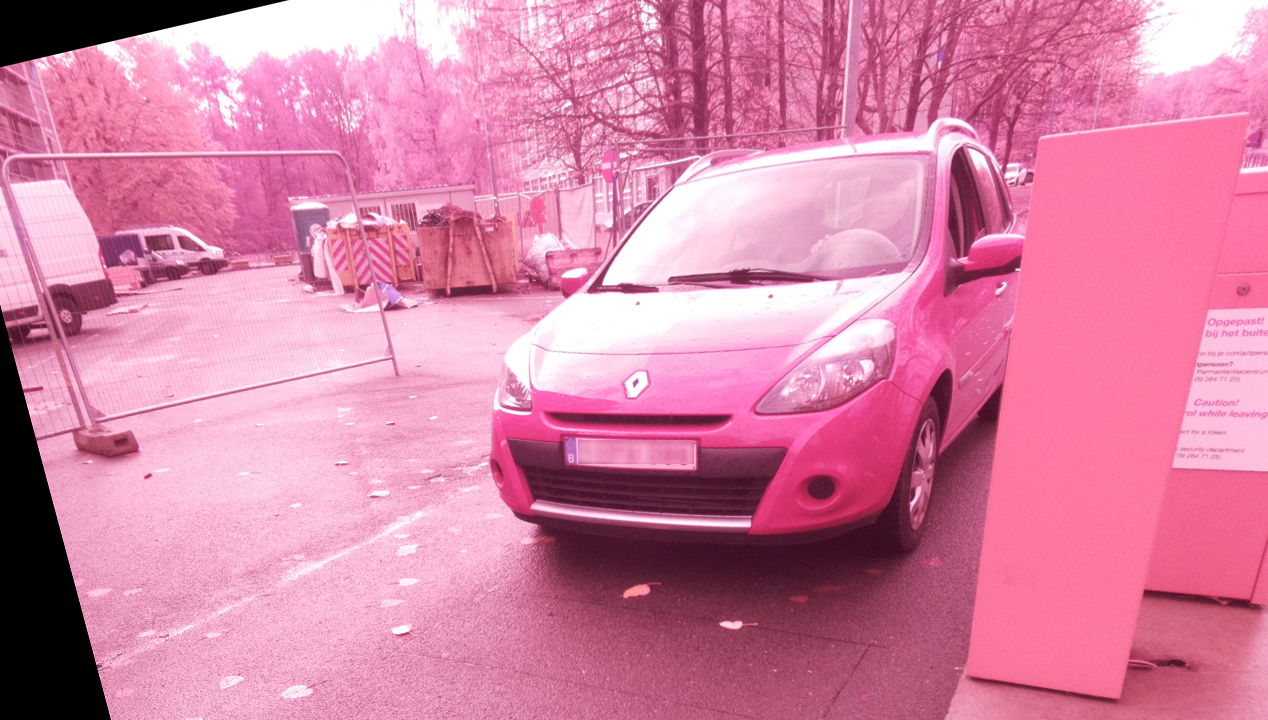
\includegraphics[width=\linewidth]{img/calibration/calibrate-cut.png}
		\caption{Gekalibreerde afbeelding}
	\end{subfigure}
	\label{fig:calibration}
	\caption{Calibratie van afbeeldingen met behulp van openalpr-utils-calibrate.}
\end{figure}

Een verduidelijking van het het verschil van de resultaten aan de uitgang van Campus Sterre - Galglaan:
\begin{table}[h!]
	\centering
	\begin{tabular}{l|l|l|l}
		 		& Incorrect & Correct & Ratio	\\ \hline
		Niet-gekalibreerd	& 25 & 2 & 7.4\%	\\
		Gekalibreerd	& 9 & 18 & 66.7\%\\
	\end{tabular}
\end{table}

\subsection{Patroon matching van nummerplaten}
Nummerplaten kunnen soms foutief gedetecteerd worden door letters en nummers die op elkaar lijken. Zo is er maar een klein verschil tussen de O, 0 en Q. 
Hierdoor kan het zijn dat een nummerplaat zoals 1-NOP-123 gelezen wordt als 1-N0P-123. In de gevallen dat deze de structuur van de reeksen tekens in de nummerplaten verhinderen, kunnen deze gemakkelijk opgelost worden door gebruik van OpenALPR's patroon matching.

Wat patroon matching doet is zoals de naam zegt; het controleren of een bekomen nummerplaat voldoet aan een bepaald patroon. In Belgie en nederland zijn deze sinds 2010 een 1 met 3 letters en 3 cijfers.

\section{Resultaten}

\subsection{Campus Sterre - Uitgang Galglaan}

De resultaten voor de uitgang van de Galglaan zijn zeer goed in vergelijking van de andere uitgangen, 22 van de 23 auto's die gepasseerd zijn, zijn correct geidentificeerd. Dit is een ratio van 95.7\%, wat een verwachte waarde is voor ANPR.

\begin{table}[h!]
	\centering
	\begin{tabular}{l|l|l|l|l}
\textbf{ANPR nauwkeurigheid: Galglaan} & Totaal & Incorrect & Correct & Ratio	\\ \hline
Per individuele foto 	& 62 & 13	& 49	& 79.0\%\\
Per auto				& 23 & 1	& 22 	& 95.7\%\\
\end{tabular}
\end{table}

\paragraph{Fouten}
De foutieve wagen, getoond in figuur \ref{foutiefgalglaan}, heeft geen opvallende geschillen dan de andere wel-gedetecteerde wagens. Qua positie, kwaliteit, focus is hij identiek. We kunnen hierdoor veronderstellen dat deze fout komt door de accuraatheid van OpenALPR zelf. Verbetering aan de uitgang lijkt niet direct nodig.
\begin{figure}[h!]
	\centering
	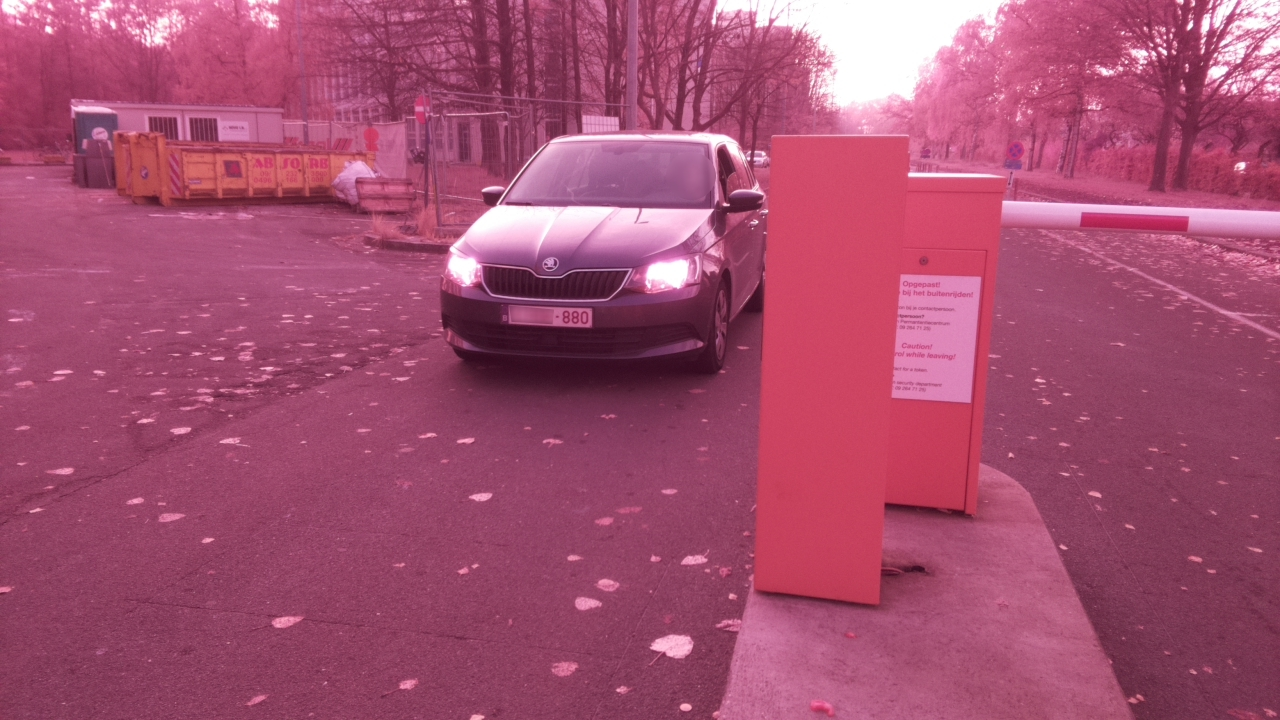
\includegraphics[width=0.5\linewidth]{img/res-galglaan/galg1.jpg}
	\caption{Niet-gedetecteerde nummerplaat aan Campus Sterre - Galglaan.}
	\label{foutiefgalglaan}
\end{figure}

\subsection{Campus Sterre - Uitgang De Pintelaan}
De uitgang op de Campus Sterre aan de De Pintelaan is de hoofduitgang van UGent en was het moeilijkste te configureren van alle uitgangen. Deze is verbonden met drie straten die enkele grote parkings verbinden, bijgevolg wordt deze het meest gebruikt van alle uitgangen. Het is dan ook belangrijk dat hier een goede detectie is.

Door de vele verbindingen is het mogelijk om de parking op allerlei manieren te bereiken, deze zijn te zien op figuur \ref{fig:satellietdepintelaan}. Dit is op zich geen probleem, maar hierdoor moet de nummerplaatdetectie wel in een groot aantal orientaties werken.

Aangezien aan deze uitgang niet direct een optimale camerahoek gevonden was, worden in de volgende onderdelen de geteste camerahoeken beschreven tesamen met hun resultaten.

\begin{figure}[h!]
	\centering
	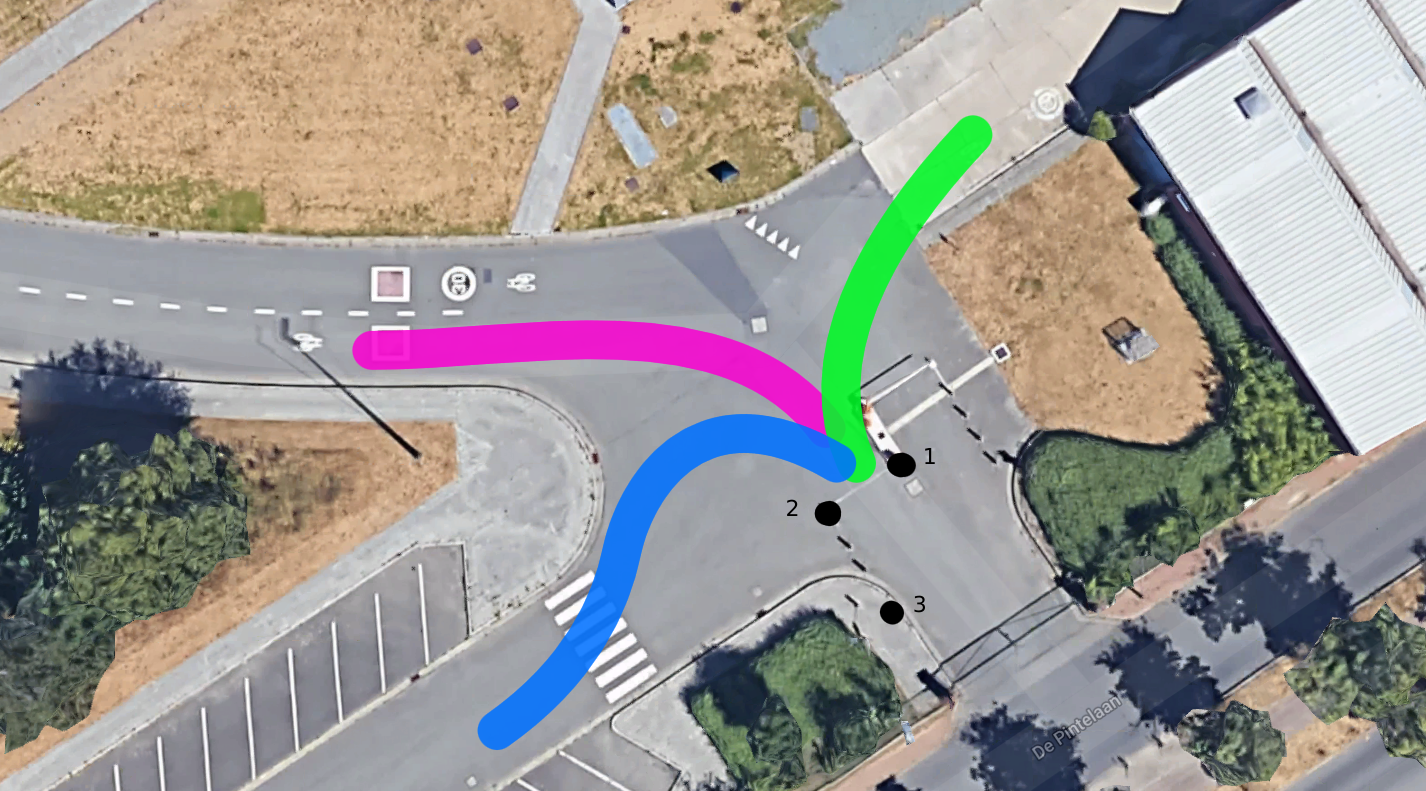
\includegraphics[width=\linewidth]{img/satellietdepintelaan.png}
	\caption{Satellietafbeelding van de Campus Sterre - Uitgang De Pintelaan met aangeduide routes en cameralocaties. \autocite{ugent2019google}}
	\label{fig:satellietdepintelaan}
\end{figure}

\subsubsection{Positie rechts van de hefboom}
In een eerste poging tot detectie werd de camera op de metalen constructie van de hefboom geplaatst, wat aan andere uitgangen al degelijke resultaten leverde. Spijtig genoeg was deze locatie duidelijk niet geschikt, de zon speelde een grote invloed op de afbeeldingen en ook de vele inrijrichtingen maakten dit moeilijk. Deze plaatsing is aangeduid op Afbeelding \ref{fig:satellietdepintelaan} als punt 1. Figuur \ref{fig:plaatsingdepintelaanorigineel} verduidelijkt de specifieke plaatsing van de camera zelf.

\begin{figure}[h!]
	\centering
	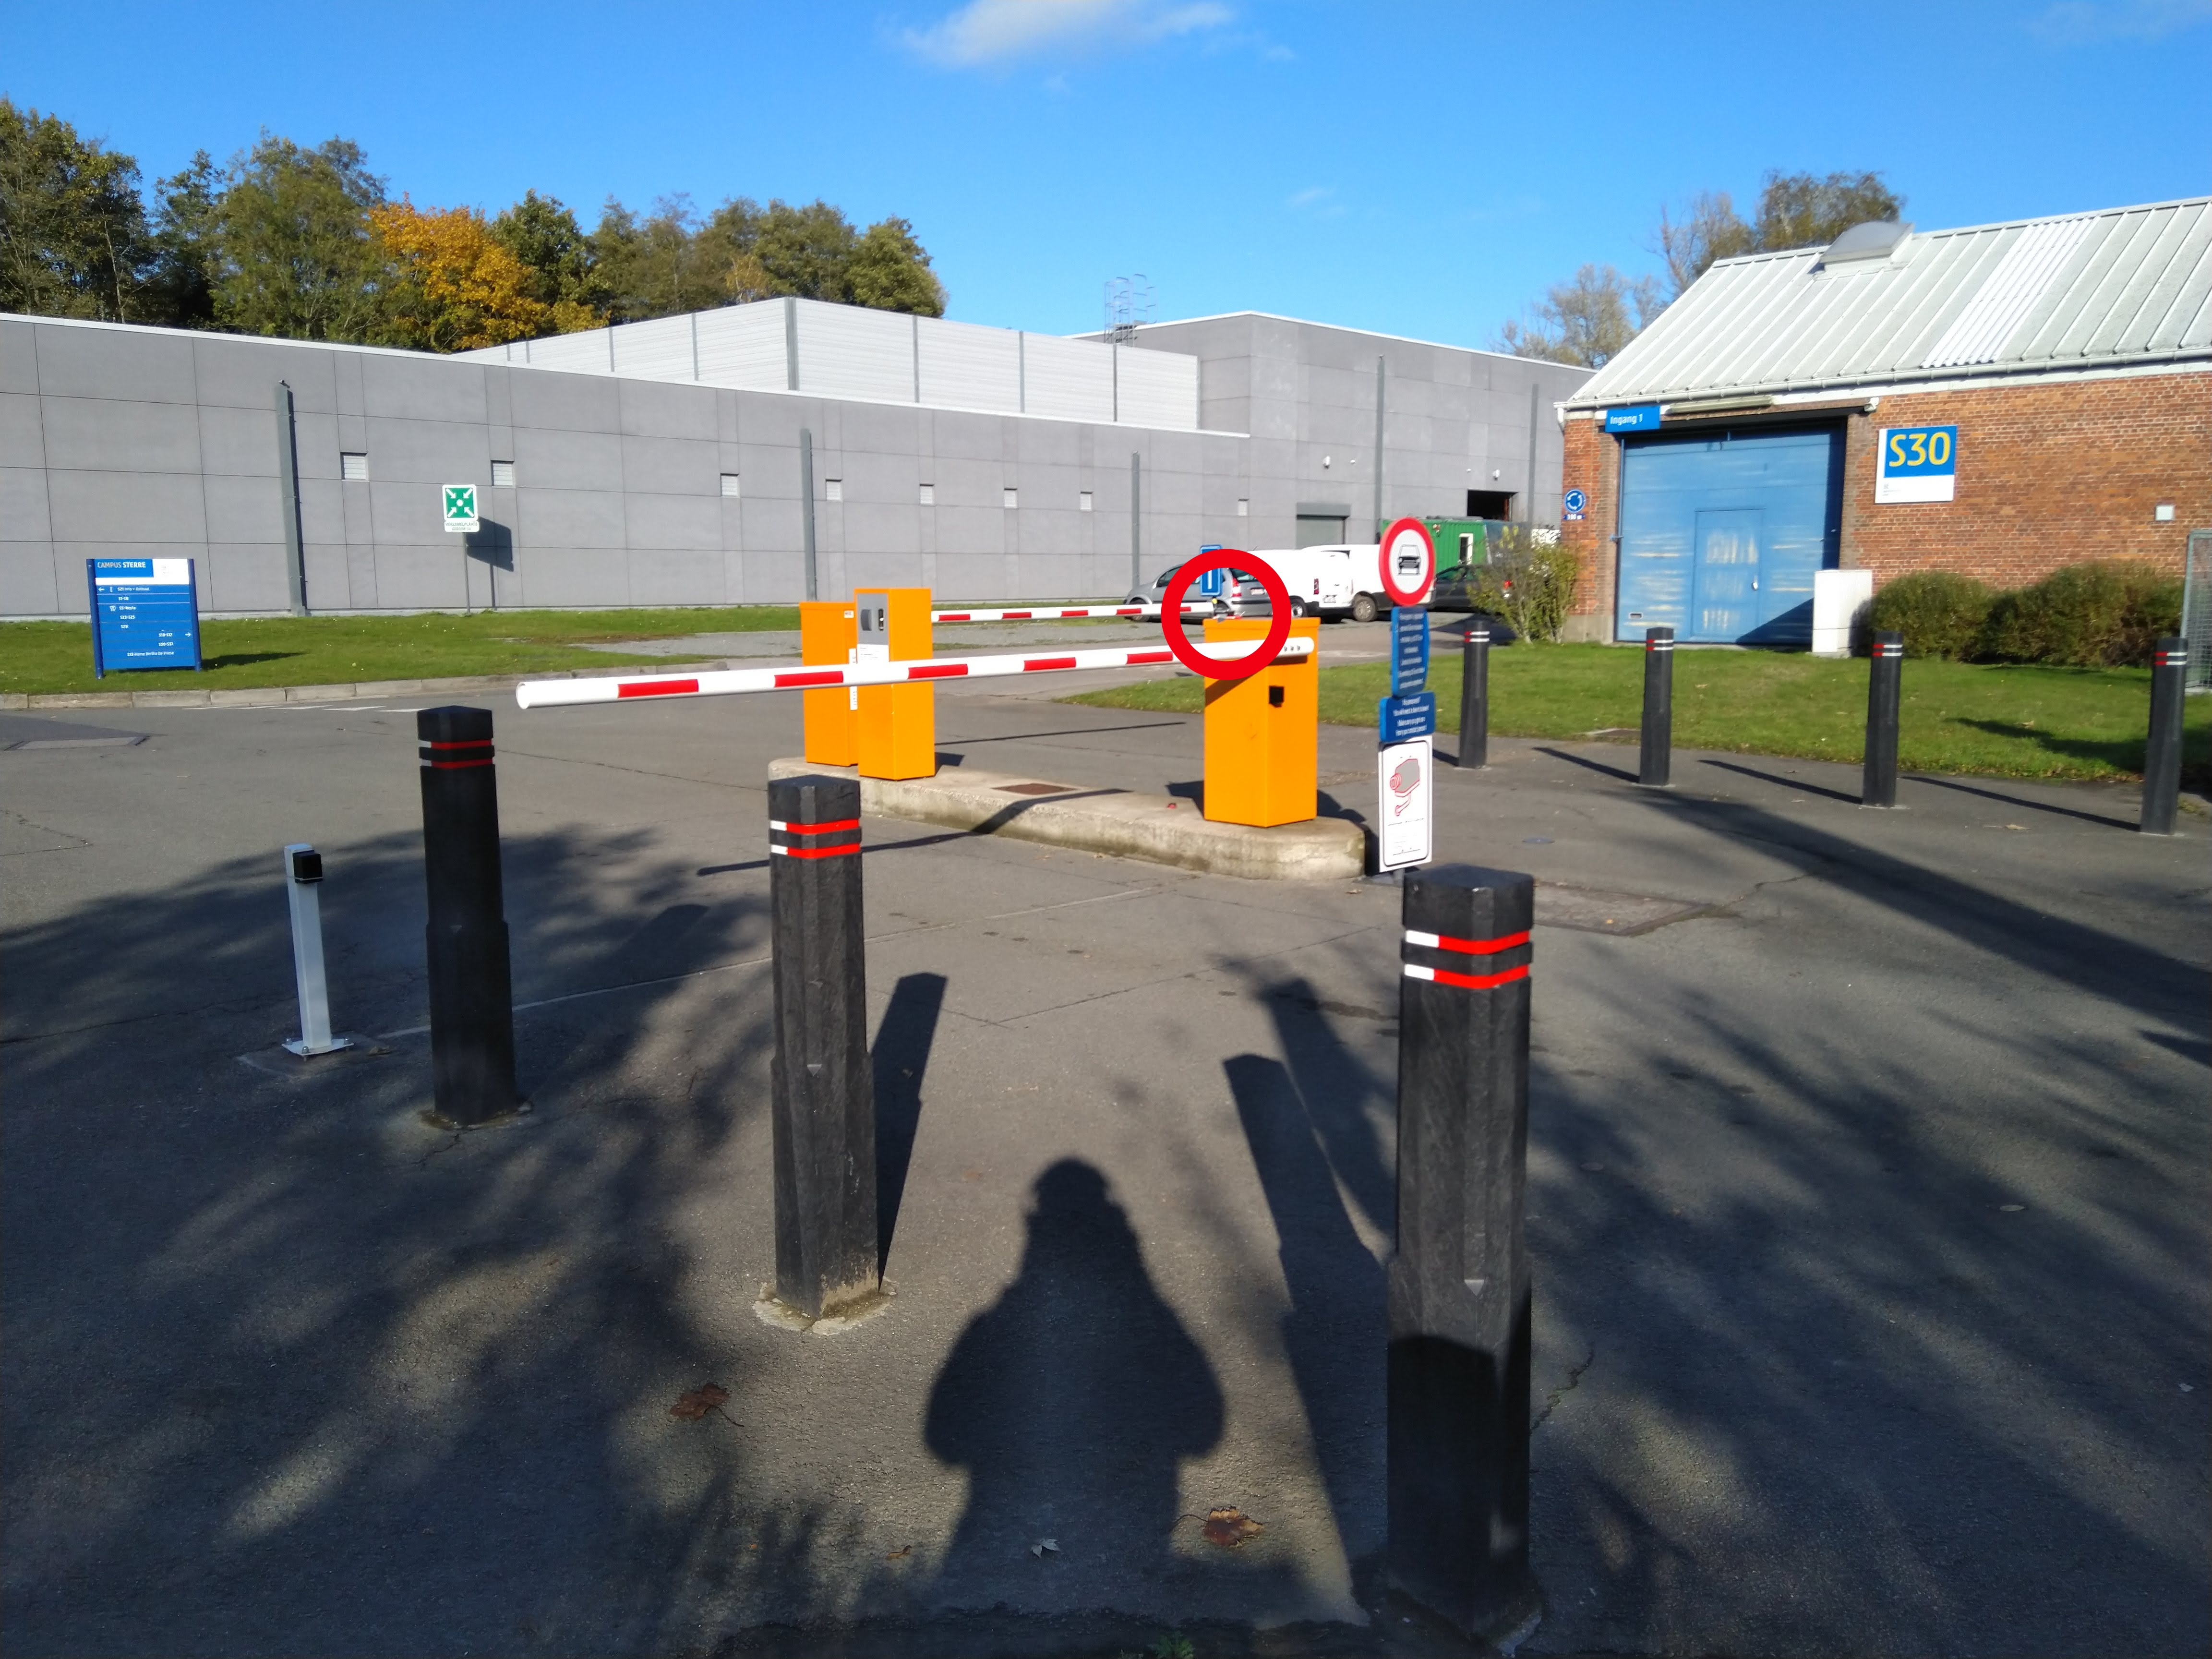
\includegraphics[width=0.8\linewidth]{img/depintelaanorigineel.jpg}
	\caption{Cameraplaatsing aan de rechterkant van de hefboom op Campus Sterre - De Pintelaan. De locatie van de camera is aangeduid met een rode cirkel.}
	\label{fig:plaatsingdepintelaanorigineel}
\end{figure}

Dit zijn de bekomen resultaten na het kalibreren van de camera:
\begin{table}[h!]
	\centering
	\begin{tabular}{l|l|l|l|l}
		\textbf{ANPR nauwkeurigheid: De Pintelaan, rechts} & Totaal & Incorrect & Correct & Ratio	\\ \hline
		Per individuele foto 	& 73 & 43	& 30	& 41.1\%\\
		Per auto				& 25 & 8	& 17 	& 68.0\%\\
	\end{tabular}
\end{table}

De eerste resultaten aan deze uitgang waren niet denderend, indien 30\% van de bezoekers terug moeten keren om toch een token te halen doet nummerplaatdetectie meer kwaad dan goed. Na het inspecteren van de foutieve afbeelding werd duidelijk dat bij vele voertuigen 's middags een grote interferentie van het zonlicht hadden. Wanneer de zon hoog staat reflecteerde het zonlicht via de nummerplaat recht in de camera, wat het contrast van de tekst op de nummerplaat in grote mate verminderde en de detectie onmogelijk maakte. Hieruit kunnen we afleiden dat deze specifieke cameraplaatsing niet geschikt is voor de uitgang en een andere camerahoek gezocht moest worden. 

Een voorbeeld van deze interferentie is te zien op Figuur \ref{SterreZonlicht}. Deze afbeelding is niet bewerkt, de nummerplaat is gewoonweg helemaal niet zichtbaar door de reflectie van het zonlicht.
\begin{figure}[h!]
	\centering
	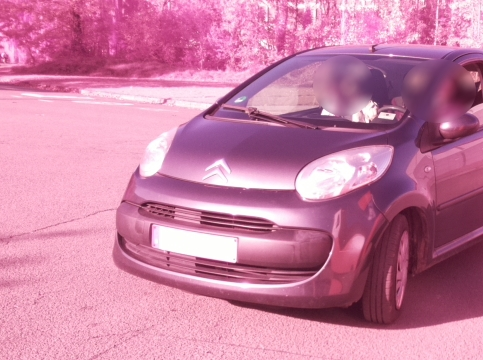
\includegraphics[width=0.8\linewidth]{img/sterre2zon.jpg}
	\caption{Interferentie van zonlicht op de parking van Campus Sterre - De Pintelaan.}
	\label{SterreZonlicht}
\end{figure}

\subsubsection{Positie links van de hefboom}
In een poging om de invloed van de zon tegen te gaan is geprobeerd om de camera aan de linkerkant van de slagboom te zetten, maar ook op deze positie maakte de zon de nummerplaten in vele gevallen minder leesbaar, bijkomend gaf de camerahoek zelf enkele nadelen. Door de vele inrijrichtingen van de auto, aangeduid op figuur \ref{fig:satellietdepintelaan}, waren een groot deel van de nummerplaten helemaal niet zichtbaar. Enkele voorbeelden hiervan zijn te zien in figuur \ref{fig:sterre-links}, Auto's die van links komen hun nummerplaten staan te schuin om soms zelfs duidelijk met het oog te kunnen lezen.

\begin{figure}[h!]
	\centering
	\begin{subfigure}[b]{0.4\linewidth}
		\includegraphics[width=\linewidth]{img/sterlinks/sterrelinks1.jpg}
	\end{subfigure}
	\begin{subfigure}[b]{0.4\linewidth}
		\includegraphics[width=\linewidth]{img/sterlinks/sterlinks2.jpg}
	\end{subfigure}
	\caption{Moeilijk te detecteren nummerplaten door scherpe camerahoek.}
	\label{fig:sterre-links}
\end{figure}

Hierdoor verkrijgen we volgende resultaten:
\begin{table}[h!]
	\centering
	\begin{tabular}{l|l|l|l|l}
		\textbf{ANPR nauwkeurigheid: De Pintelaan, links} & Totaal & Incorrect & Correct & Ratio	\\ \hline
		Per individuele foto 	& 50 & 31	& 19	& 38.0\%\\
		Per auto				& 17 & 8	& 9 	& 52.9\%\\
	\end{tabular}
\end{table}

Met een slechter resultaat dan de vorige positie en net meer dan de helft van de auto's correct te kunnen detecteren, kunnen we besluiten dat deze positie geen oplossing is.

\subsubsection{Positie achteraan de uitgang}
Als derde optie is er getest op de mogelijkheid om van een verdere locatie foto's te nemen aan de hand van een statief om de camera op een geschikte hoogte te houden. Dit is aangetoond op figuur \ref{plaatsingdepintelaan}. Door de camera naar achteren te zetten zorgen de inrijrichtingen tot geen problemen meer aangezien de wagens allemaal op dezelfde plaats kunnen gefotografeerd worden. Verder is er geen storing meer van het zonlicht omdat de camera naar omlaag is gericht.

Deze positie is een drie meter naar achteren van de linkerkant van de hefboom, dit zodat da invalshoek van de camera zo klein mogelijk blijft. De hoogte van de camera is 1,5 meter hoog, wat hoog genoeg was om de invloed van het zonlicht weg te werken.
\begin{figure}[h!]
	\centering
	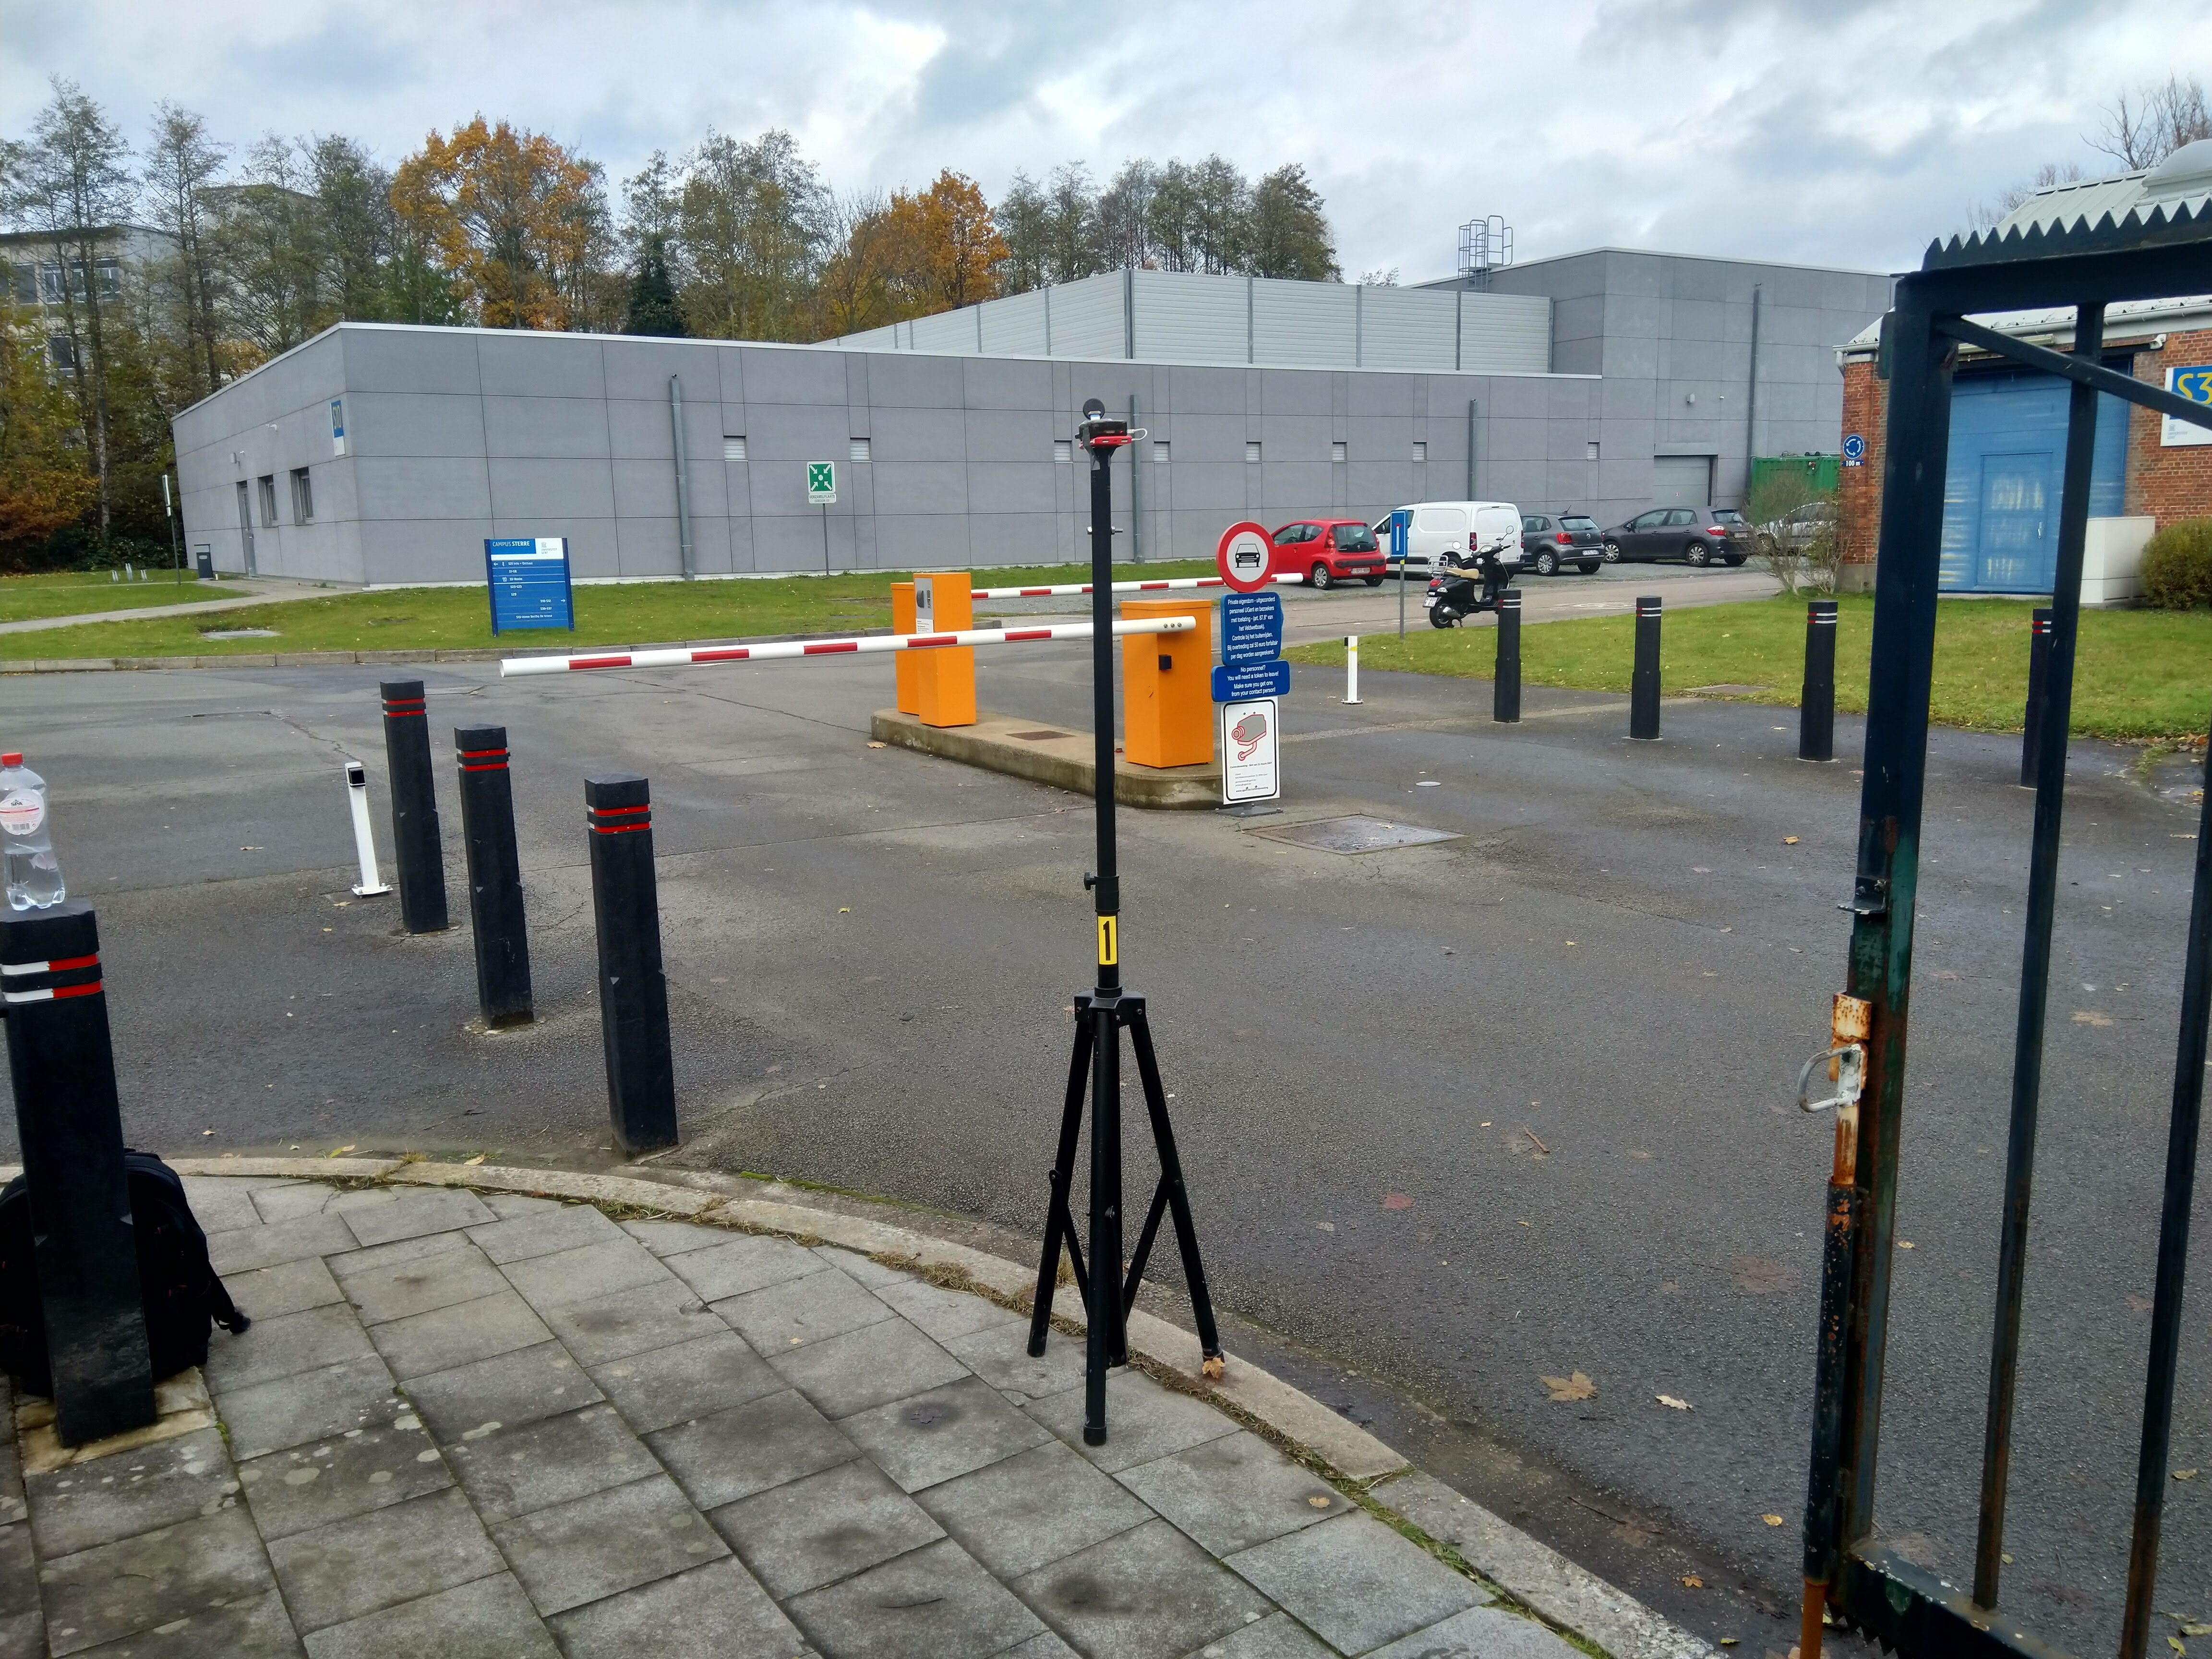
\includegraphics[width=0.8\linewidth]{img/depintelaanstatief.jpg}
	\caption{Cameraplaatsing met statief op Campus Sterre - De Pintelaan.}
	\label{plaatsingdepintelaan}
\end{figure}

Volgende resultaten zijn bekomen aan de uitgang:
\begin{table}[h!]
	\centering
	\begin{tabular}{l|l|l|l|l}
		\textbf{ANPR nauwkeurigheid: De Pintelaan, achteraan} & Totaal & Incorrect & Correct & Ratio	\\ \hline
		Per individuele foto 	& 75 & 35	& 40	& 53.3\%\\
		Per auto				& 24 & 6	& 18 	& 75.0\%\\
	\end{tabular}
\end{table}

Deze locatie is een verbetering tov. de vorige posities. Allereerst staan alle auto's op dezelfde locatie ongeacht van inrijrichting. Dit maakt de configuratie van OpenALPR een pak aangenamer en betrouwbaarder.

Ondanks deze voordelen is de nauwkeurigheid niet hoog genoeg en zijn er toch 6 auto's die niet gedetecteerd zijn. Na deze na foto's te gaan is het duidelijk dat dit komt door de grote afstand en bijgevolg lagere resolutie van de nummerplaten. Een voorbeeld hiervan is te zien op figuur \ref{fig:lowressterre}.

\begin{figure}[h!]
	\centering
	\begin{subfigure}[b]{0.49\linewidth}
		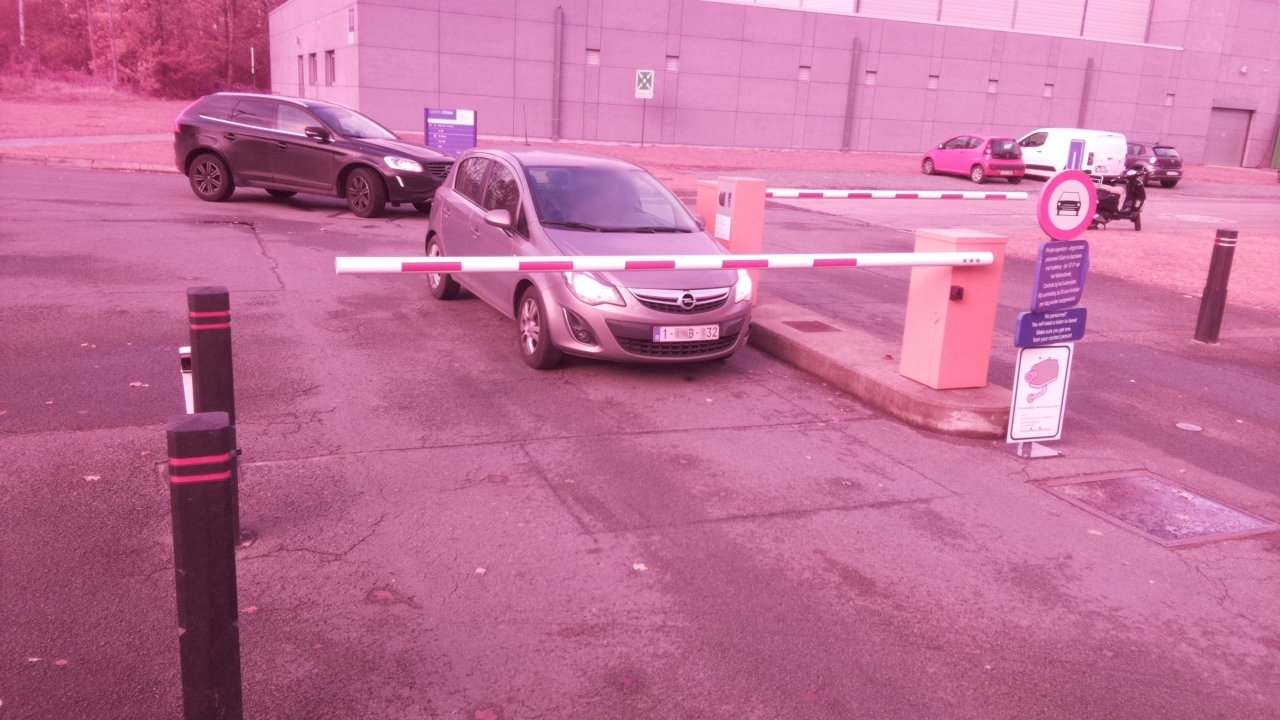
\includegraphics[width=\linewidth]{img/sterachter/sterachter1.jpg}
	\end{subfigure}
	\begin{subfigure}[b]{0.49\linewidth}
		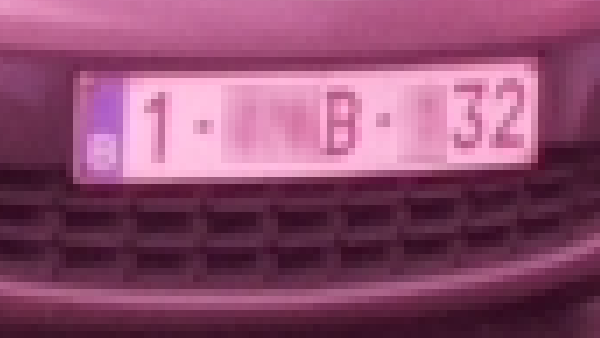
\includegraphics[width=\linewidth]{img/sterachter/sterachter2.png}
	\end{subfigure}
	\caption{Moeilijk te detecteren nummerplaten door een te lage resolutie. Enkele karakters zijn onduidelijk gemaakt uit privacy van de bestuurder.}
	\label{fig:lowressterre}
\end{figure}

Verder is één voertuig niet gedetecteerd niet door de lage resolutie maar door de hoogte van de slagboom, deze vrachtagen zijn nummerplaat is te hoog aan het voertuig gemonteerd waardoor de slagboom ervoor staat op de foto. Dit is te zien in figuur \ref{fig:slagboomster}. Deze situatie is wellicht uitzonderlijk. Alle andere auto's hun nummerplaat zit ruim onder de slagboom.

\begin{figure}[h!]
	\centering
	\begin{subfigure}[b]{0.99\linewidth}
		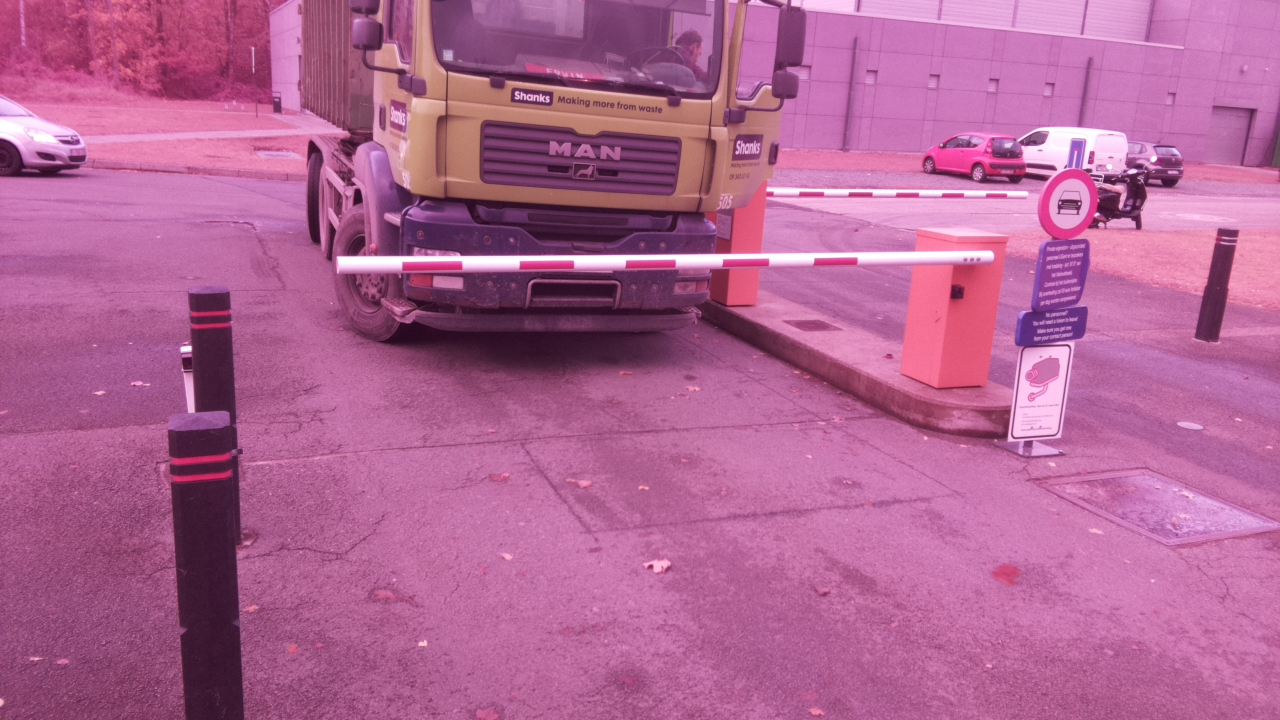
\includegraphics[width=\linewidth]{img/sterachter/sterachter3.jpg}
	\end{subfigure}
	\caption{Niet te detecteren nummerplaat omwille van slagboom die het zicht verhindert.}
	\label{fig:slagboomster}
\end{figure}

\subsubsection{Positie achteraan de uitgang - hoge resolutie}
Ten laatste is het onderzoek op de vorige locatie opnieuw uitgevoerd. De nauwkeurigheid van de PiNoIR camera biedt echter een veel hogere resolutie aan. Dit maakte het mogelijk om softwarematig in te zoomen op de foto's met een betere kwaliteit. In afbeelding \ref{fig:ressterrecomparison} is dit verschil van de foto's duidelijk te zien.

\begin{figure}[h!]
	\centering
	\begin{subfigure}[b]{0.49\linewidth}
		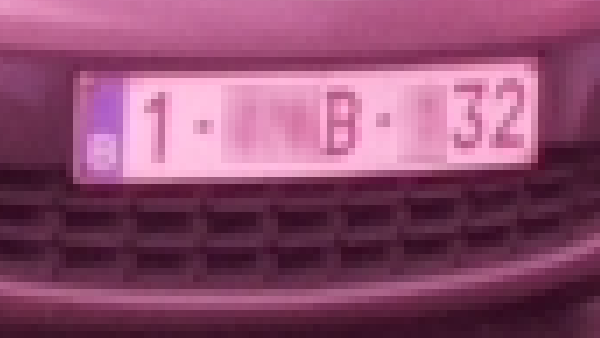
\includegraphics[width=\linewidth]{img/sterachter/sterachter2.png}
		\caption{Originele kwaliteit}
	\end{subfigure}
	\begin{subfigure}[b]{0.49\linewidth}
		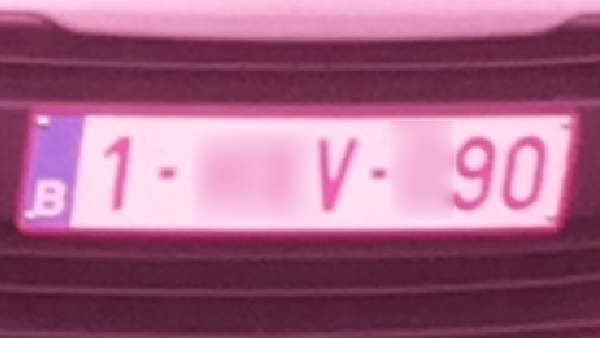
\includegraphics[width=\linewidth]{img/sterachter/hressmall2.png}
		\caption{Verhoogde kwaliteit}
	\end{subfigure}
	\caption{Verhoogde nauwkeurigheid door het inzoomen van de camera.}
	\label{fig:ressterrecomparison}
\end{figure}

Na de camera vervolgens opnieuw te kalibreren zijn volgende resultaten bekomen:
\begin{table}[h!]
	\centering
	\begin{tabular}{l|l|l|l|l}
		\textbf{ANPR nauwkeurigheid: De Pintelaan, achteraan} & Totaal & Incorrect & Correct & Ratio	\\ \hline
		Per individuele foto 	& 19 & 45	& 64	& 70.3\%\\
		Per auto				& 2 & 24	& 26 	& 92.0\%\\
	\end{tabular}
\end{table}

Deze zijn een enorm verschil met het vorig resultaat van 75\% van de vorige foto's en bieden een haalbare oplossing voor de uitgang van de De Pintelaan.

\paragraph{Nadelen}
Indien een camera op deze locatie moet gezet worden zullen er enkele maatregelingen nodig zijn om de camera te plaatsen en van stroom te voorzien. Een paal zou in de straat moeten vastgezet worden en een reeks kabels voor stroom en data moeten naar de metalen constructie van de hefboom lopen. Dit vraagt een redelijke hoeveelheid meer werk en kosten dan een systeem dat op de behuizing zelf staat.

\paragraph{Verbeteringen}
De camera is niet direct te hoog geplaatst, dit was uit voorzorg dat de hefboom van de toegang het beeld van de nummerplaten overlapt. Na de foto's te analyseren bleek het toch dat er nog ruim veel plaats was om de camera hoger te zetten. Dit is een vereiste om mogelijkse voorbijgangers te beletten van vandalisme. Er wordt verondersteld dat het verhogen van de camera geen direct negatieve invloed op de resultaten zal hebben, dit zolang de kalibratie opnieuw wordt uitgevoerd.

\subsection{Campus Coupure - Uitgang Kruisboogstraat}

Volgende resultaten zijn bekomen voor de uitgang van de Kruisboogstraat:

\begin{table}[h!]
	\centering
	\begin{tabular}{l|l|l|l|l}
		\textbf{ANPR nauwkeurigheid: Kruisboogstraat} & Incorrect & Correct & Totaal & Ratio	\\ \hline
		Per individuele foto 	& 68 & 16	& 52	& 76.5\%\\
		Per auto				& 25 & 1	& 26 	& 96.15\%\\
	\end{tabular}
	\label{ResultatenKruisboog}
\end{table}

\subsubsection{Fouten}
Op 1 auto na zijn alle auto's correct geïdentificeerd. De incorrecte afbeeldingen hebben geen merkwaardige verschillen van de andere afbeeldingen waardoor de juistheid lager zou liggen. We kunnen hieruit dus veronderstellen dat deze fout komt door de nauwkeurigheid van OpenALPR zelf.

\subsection{Campus Coupure - Uitgang Coupure Links}
De uitgang aan de Coupure Links had niet genoeg doorrijdende auto's om een degelijke steekproef te nemen of een correcte cameraconfiguratie te vinden. Hierdoor zal deze uitgang niet verder verwerkt worden in dit onderzoek.

\subsection{Algemene resultaten}
In het donker is de interferentie van de koplampen niet te groot, maar de algemene donkerheid van de omgeving zorgt ervoor dat de raspberry pi zijn shutter te lang openhoudt en dat de afbeeldingen enorm donker blijken. Het is dus vereist om extra infraroodbelichting bij te plaatsen.
\begin{figure}[h!]
	\centering
	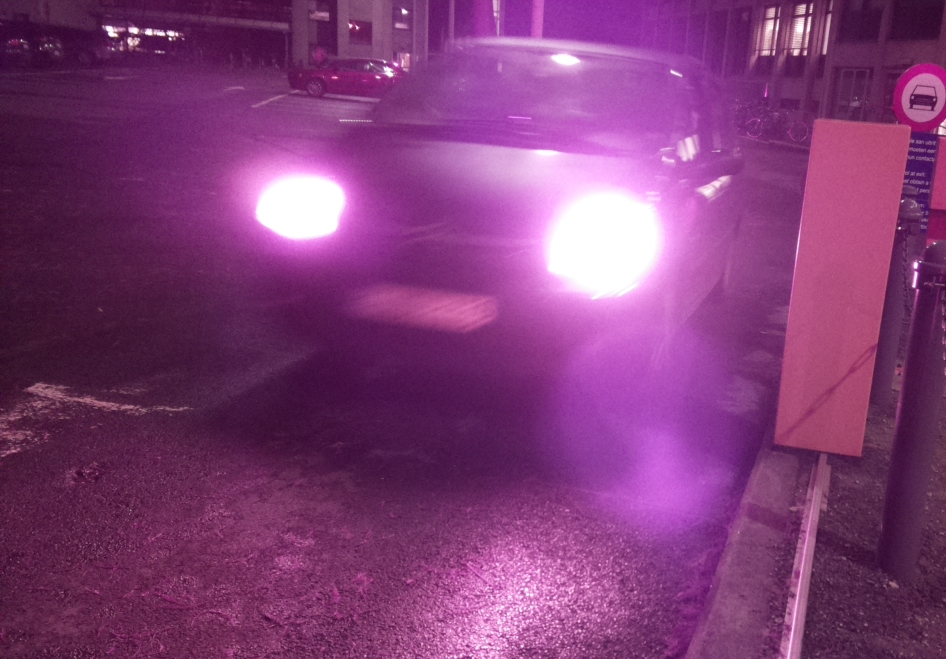
\includegraphics[width=0.5\linewidth]{img/nacht-coupure.jpg}
	\caption{Onnauwkeurige foto's door een tekort aan licht.}
	\label{SterreDonker}
\end{figure}

\begin{table}[h!]
	\centering
	\begin{tabular}{l|l|l|l|l}
		\textbf{Resultaten per individuele foto}	& \textbf{Incorrect}	& \textbf{Correct} & \textbf{Aantal foto's} & \textbf{Ratio} \\ \hline
		Campus Coupure - Uitgang Kruisboogstraat & 16 & 52 & 68 & 76.5\% \\
		Campus Sterre - Uitgang Galglaan 		 & 13 & 49 & 62 & 79.0\%\\
		Campus Sterre - Uitgang De Pintelaan	 & 19 & 45 & 64 & 70.3\%\\ \hline
		Totaal 									 & 48 & 146 & 194 & 75.3\%
	\end{tabular}
\end{table}

\begin{table}[h!]
	\centering
	\begin{tabular}{l|l|l|l|l}
		\textbf{Resultaten per auto} & \textbf{Incorrect}	& \textbf{Correct} & \textbf{Aantal auto's} & \textbf{Ratio} \\ \hline
		Campus Coupure - Uitgang Kruisboogstraat& 1 & 25  & 26 & 96.15\% \\
		Campus Sterre - Uitgang Galglaan		& 1 & 22  & 23 & 95.7\%\\
		Campus Sterre - Uitgang De Pintelaan	& 2 & 24  & 26 & 92.0\%\\ \hline
		Totaal 									& 4 & 71 & 75 & 94.7\%
	\end{tabular}
\end{table}


\paragraph{Verbeteringen}\
96.15\% is op zich een geslaagde waarde voor nummerplaatdetectie. Indien men toch de accuraatheid wilt verbeteren is de beste optie in de investering van de betalende versie van OpenALPR.

\section{Conclusie}
Op 2 van de 3 uitgangen zijn een nauwkeurigheid boven 95\% bereikt. Op deze uitgangen kunnen we aannemen dat nummerplaatdetectie op zich al mogelijk is. De derde uitgang aan de sterre heeft een te lage nauwkeurigheid van 75\%. Indien 1 op 4 auto's terug naar de parking moeten rijden om toch een token te behalen doet nummerplaatdetectie meer kwaad dan goed. Rekeninghoudend met de gemiddelde nauwkeurigheid van 89\% is dit een haalbare technologie.

In dit onderzoek is niet aangegaan hoe goed deze technologie presteert in moeilijke condities zoals in de regen of 's nachts. Op basis van bestaande onderzoeken (?) wordt hier verwacht dat de resultaten lager zullen zijn dan overdag. Aangezien de resultaten overdag maar net haalbaar is zal deze 's nachts helemaal niet haalbaar zijn.

Op vlak van wetgeving en GDPR is nummerplaatdetectie dan wel weer zeker mogelijk.

\section{Uitbreidingen}
Locatie van de sensor kan mss in het midden van balk \autocite{buhus2016automatic}.